\documentclass{standalone}
\usepackage{pgfplots}
\pgfplotsset{compat=1.17}

\begin{document}

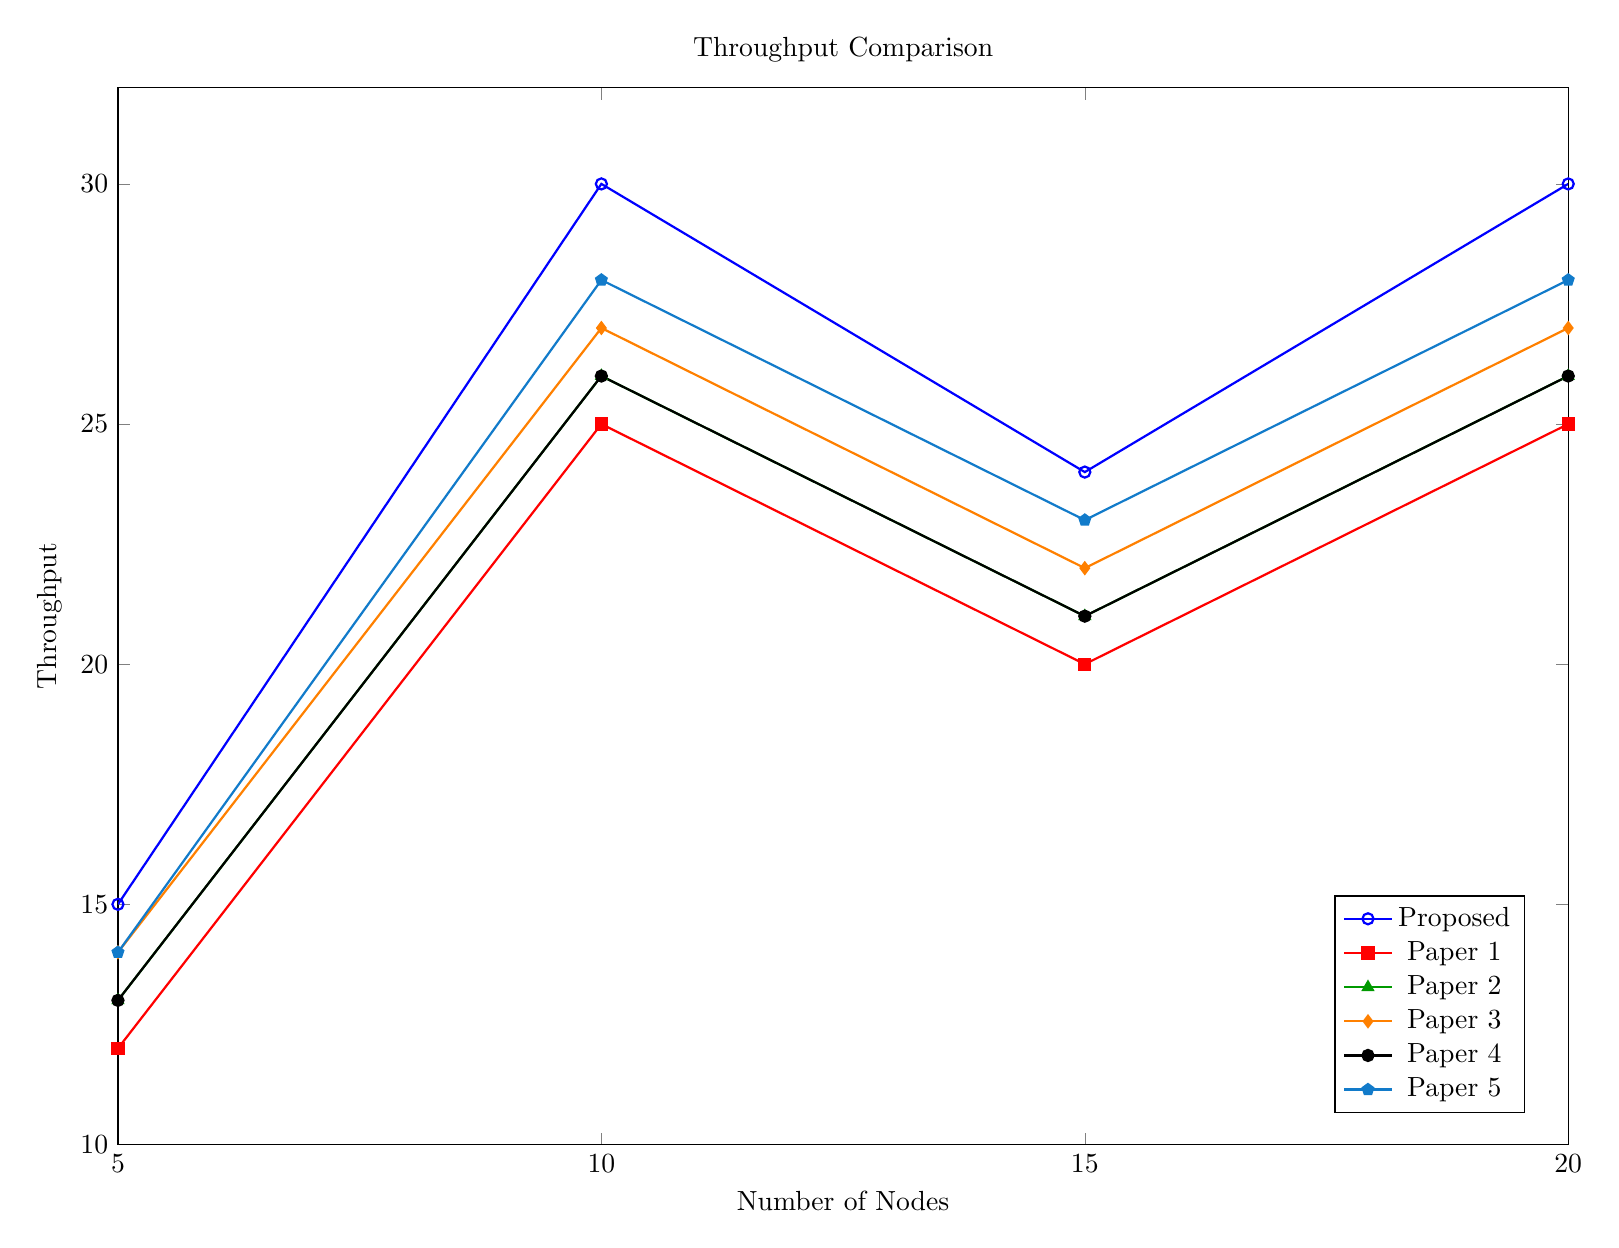
\begin{tikzpicture}
\begin{axis}[
width=20cm,
height=15cm,
title={Throughput Comparison},
xlabel={Number of Nodes},
ylabel={Throughput},
xmin=5, xmax=20,
ymin=10, ymax=32,
xtick={5,10,15,20},
ytick={10,15,20,25,30},
grid=none,
legend pos=south east
]

\addplot[color=blue, mark=o, thick] coordinates {(5,15) (10,30) (15,24) (20,30)};
\addplot[color=red, mark=square*, thick] coordinates {(5,12) (10,25) (15,20) (20,25)};
\addplot[color=green!60!black, mark=triangle*, thick] coordinates {(5,13) (10,26) (15,21) (20,26)};
\addplot[color=orange, mark=diamond*, thick] coordinates {(5,14) (10,27) (15,22) (20,27)};
\addplot[color=black, mark=*, thick] coordinates {(5,13) (10,26) (15,21) (20,26)};
\addplot[color=cyan!60!blue, mark=pentagon*, thick] coordinates {(5,14) (10,28) (15,23) (20,28)};

\legend{Proposed , Paper 1, Paper 2, Paper 3, Paper 4, Paper 5}

\end{axis}
\end{tikzpicture}

\end{document}